% catalogue: title = Commutative diagram drawn with nodes
% catalogue: min-coverage = 1.00
\documentclass[border=10pt]{standalone}
\PassOptionsToPackage{dvipsnames,svgnames,x11names}{xcolor}
\usepackage{tikz}
\usepackage{pgfplots}
\pgfplotsset{compat=newest}
\usepgfplotslibrary{groupplots}
\usetikzlibrary{arrows.meta}
\begin{document}
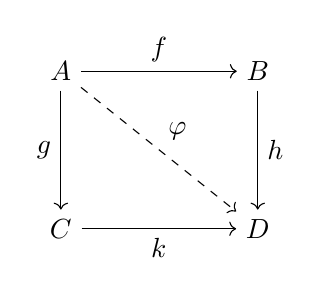
\begin{tikzpicture}
    \node (A) at (0, 2) {$A$};
    \node (B) at (2.5, 2) {$B$};
    \node (C) at (0, 0) {$C$};
    \node (D) at (2.5, 0) {$D$};
    \draw[->] (A) -- node[above] {$f$} (B);
    \draw[->] (A) -- node[left] {$g$} (C);
    \draw[->] (B) -- node[right] {$h$} (D);
    \draw[->] (C) -- node[below] {$k$} (D);
    \draw[->, dashed] (A) -- node[above right] {$\varphi$} (D);
\end{tikzpicture}
\end{document}
